\documentclass[usenames,dvipsnames,10pt,aspectratio=169]{beamer} 

\usepackage[utf8]{inputenc}
\usepackage{verbatim}
\usepackage{minted}
\usepackage{graphicx}
\usepackage{wrapfig}
\usepackage{geometry}
\usepackage{listings}
% \usepackage{showframe}
\usepackage{enumitem}
\usepackage{color, xcolor}
\usepackage[document]{ragged2e}
\usetheme{umu}

\usemintedstyle{monokai}

\usepackage{hyperref}
\hypersetup{
    colorlinks=true,
    linkcolor=ucugreyish,
    filecolor=ucured,
    urlcolor=ucublue,
}
\urlstyle{same}

%%% Some useful commands
% pdf-friendly newline in links
\newcommand{\pdfnewline}{\texorpdfstring{\newline}{ }} 
% Fill the vertical space in a slide (to put text at the bottom)
\newcommand{\framefill}{\vskip 0pt plus 1 filll}

%%% Enter additional packages below (or above, I can't stop you)! / Jesper
\renewcommand{\proofname}{\sffamily{Proof}}

% presentation template slides usage
% \framecard[color (not working)]{textbuf}
% \framesplit{Header}{picture}{textbuf}
% \framepic{image}{text}
% \lstinputlisting[language=Bash, style=codestyle]{code/namespace_ex.sh}

%%%%%%%%%%%%%%%%%%%%%%%%%%%%%%%%%%%%%%%%%%%%%%%%%%%%%%%%%%%%%%%%%%%%%%%%%%%%%%%%%%%%%
\title{Linux course}
\subtitle{Tools overview}
\date[\today]{\small\today}
\author[Morhunenko Mykola]{Morhunenko Mykola}
\institute{APPS@UCU}

\setlist[itemize, 1]{label=$\color{ucublue} \bullet$, leftmargin=-2mm}

\begin{document}

\begin{frame}
\titlepage
\end{frame}

\begin{frame}{\contentsname}
    \setbeamercolor{background canvas}{bg=ucugrey}
    \tableofcontents
\end{frame}

\begin{frame}
    \frametitle{Intro}
    \begin{itemize}
        \item In this presentation, we will overview some tools that are available on all Linux distributions
        \item All of them have a high barrier to entry as Linux itself, but when you are there - you will not imagine your life without that tools
        \item Example: it's not a one-day task to learn how to move around your system, but after few months of practice working with CLI, GUI for you will be as slow as a turtle is slow in comparison with a rabbit
    \end{itemize}
\end{frame}

\section{Shell}
{ % all template changes are local to this group.
    \setbeamertemplate{navigation symbols}{}
    \begin{frame}<article:0>[plain]
        \begin{tikzpicture}[remember picture,overlay]
            \node[at=(current page.center)] {
                
\includegraphics[keepaspectratio,width=\paperwidth]{graphics/shell.jpg}
            };
        \end{tikzpicture}
     \end{frame}
}

\begin{frame}{The most important tool}
    \begin{itemize}
        \item The most important tool, what makes\ex{Linux} over\ex{Windows}is its command shell, and\ex[ucuorange]{every computer scientist}should know how to use it
        \item In Linux,\ex{everything is a file}, this approach makes possible automation and scripting of everyday tasks. Shell gives you unlimited power over your system
        \item Only with everyday practice it is possible to improve both work quality and speed
        \item But\ex{sh}itself is hard to use, and very slow.\ex{Bash}aslo is not the best, so what to use?
        \item\ex{ZSH}with\ex{oh-my-zsh}is the best choice of our days
        \item It allows to use\ex{autocompletion},\ex{syntax highlight}and git information (as a branch, each file's status etc.) and a lot of more advanced features
        \item Almost all tools in this presentation are using\ex{Command Line Interface (CLI)}given by shell
    \end{itemize}
\end{frame}

\section{Vim}
\framepic{graphics/vim_w.png}{}
\framesplitc{Vi}{graphics/vim_meme.png}{
    \begin{itemize}
        \item You have heard about \ex{vim}, haven't you?
        \item But let's start with \ex{vi}
        \item Vi is a part of POSIX
        \item It's CLI editor (forget that you have a mouse)
        \item There are shortcuts for everything
        \item If there is no, you can create them for yourself
        \item Every good enough 21'st century editor has an extension for a \ex{vi mode}
        \item But almost nobody uses it - only on some low memory and low power machines. So we move to vim
    \end{itemize}
}

\begin{frame}{Vim}
    \begin{itemize}
        \item \ex{Vim} stands for 'Vi IMproved'
        \item According to Linux Journal survey, 38\% (in average for 2009-2018) of respondents vote for vim as the best editor
        \item It has much more features, than \ex{vi}, including more commands, scriptable syntax highlighting and extensions, graphical interface (and mouse support, but don't use it)
        \item As \ex{vi}, it has six modes - normal, visual, insert, command-line, select, and ex (yes, not only NORMAL and INSERT)
        \item Because of a huge community (38\% of world's best geeks) \ex{vim} became a powerful IDE with thousands of extensions (syntax highlight, autocompletion, spell checking, project tree etc.)
        \item The most powerful tool of \ex{vim} is inside - its shortcuts. You can make your work dozens of times faster without a touchpad and a mouse
    \end{itemize}
\end{frame}

\begin{frame}{NeoVim}
    \begin{itemize}
        \item Neovim is just a fork of Vim with some Python extensions 
        \item And cool logo =)
        \item Also Neovim is a community-driven text editor, while Vim is a project of only one person - \ex{Bram Moolenaar}
        \item One 'expert' on reddit wrote that:
        
                \hspace*{1cm} "Neovim exists to convince Bram to push new features to Vim"
            
            And I mostly agree with him.
    \end{itemize}    
\end{frame}


\section{Tmux}
{ % all template changes are local to this group.
    \setbeamertemplate{navigation symbols}{}
    \begin{frame}<article:0>[plain]
        \begin{tikzpicture}[remember picture,overlay]
            \node[at=(current page.center)] {
                
\includegraphics[keepaspectratio,width=\paperwidth/2]{graphics/Tmux_logo.png}
            };
        \end{tikzpicture}
     \end{frame}
}

\begin{frame}{Tmux}
    \begin{itemize}
        \item \ex{TMUX} stands for Terminal MUltipleXer
        \item There are some other (screen, Konsole, etc.), but they are not so good as TMUX
        \item Why do we need it?
        \item As you continue your practice in CLI, you can notice that it is not enough to have only one terminal window
        \item With this much multitasking going on, we want to have more terminals. So people create a \ex{terminal multiplexor}
        \item What TMUX can do?
        \begin{itemize}
            \item Not only split and stack tab but also make tabs
            \item Continue running programs in the background
            \item With extensions you can write layout files in \ex{.yml} format
            \item Search through terminal output and move around with Vim shortcuts
            \item Other interesting stuff
        \end{itemize}
    \end{itemize}
\end{frame}


\framesplitc{Tmux}{graphics/tmux_explain.png}{
    \begin{itemize}
        \item A Tmux Session with two tmux tabs with multiple tmux panes within each
        \item As \ex{vim}, tmux has modes - view and command (Ctrl+b be default)
        \item Every pane has three modes - view, choose and copy
        \item To enter a \ex{copy mode} - \ex{Ctrl+b [}
        \item It allows you to use vim keys for moving around and copying text
        \item For more information see \ex{man tmux} or \href{https://man7.org/linux/man-pages/man1/tmux.1.html}{linux man page}
    \end{itemize}
}

\begin{frame}{For the very beginning:}
        \hspace{-1cm}
        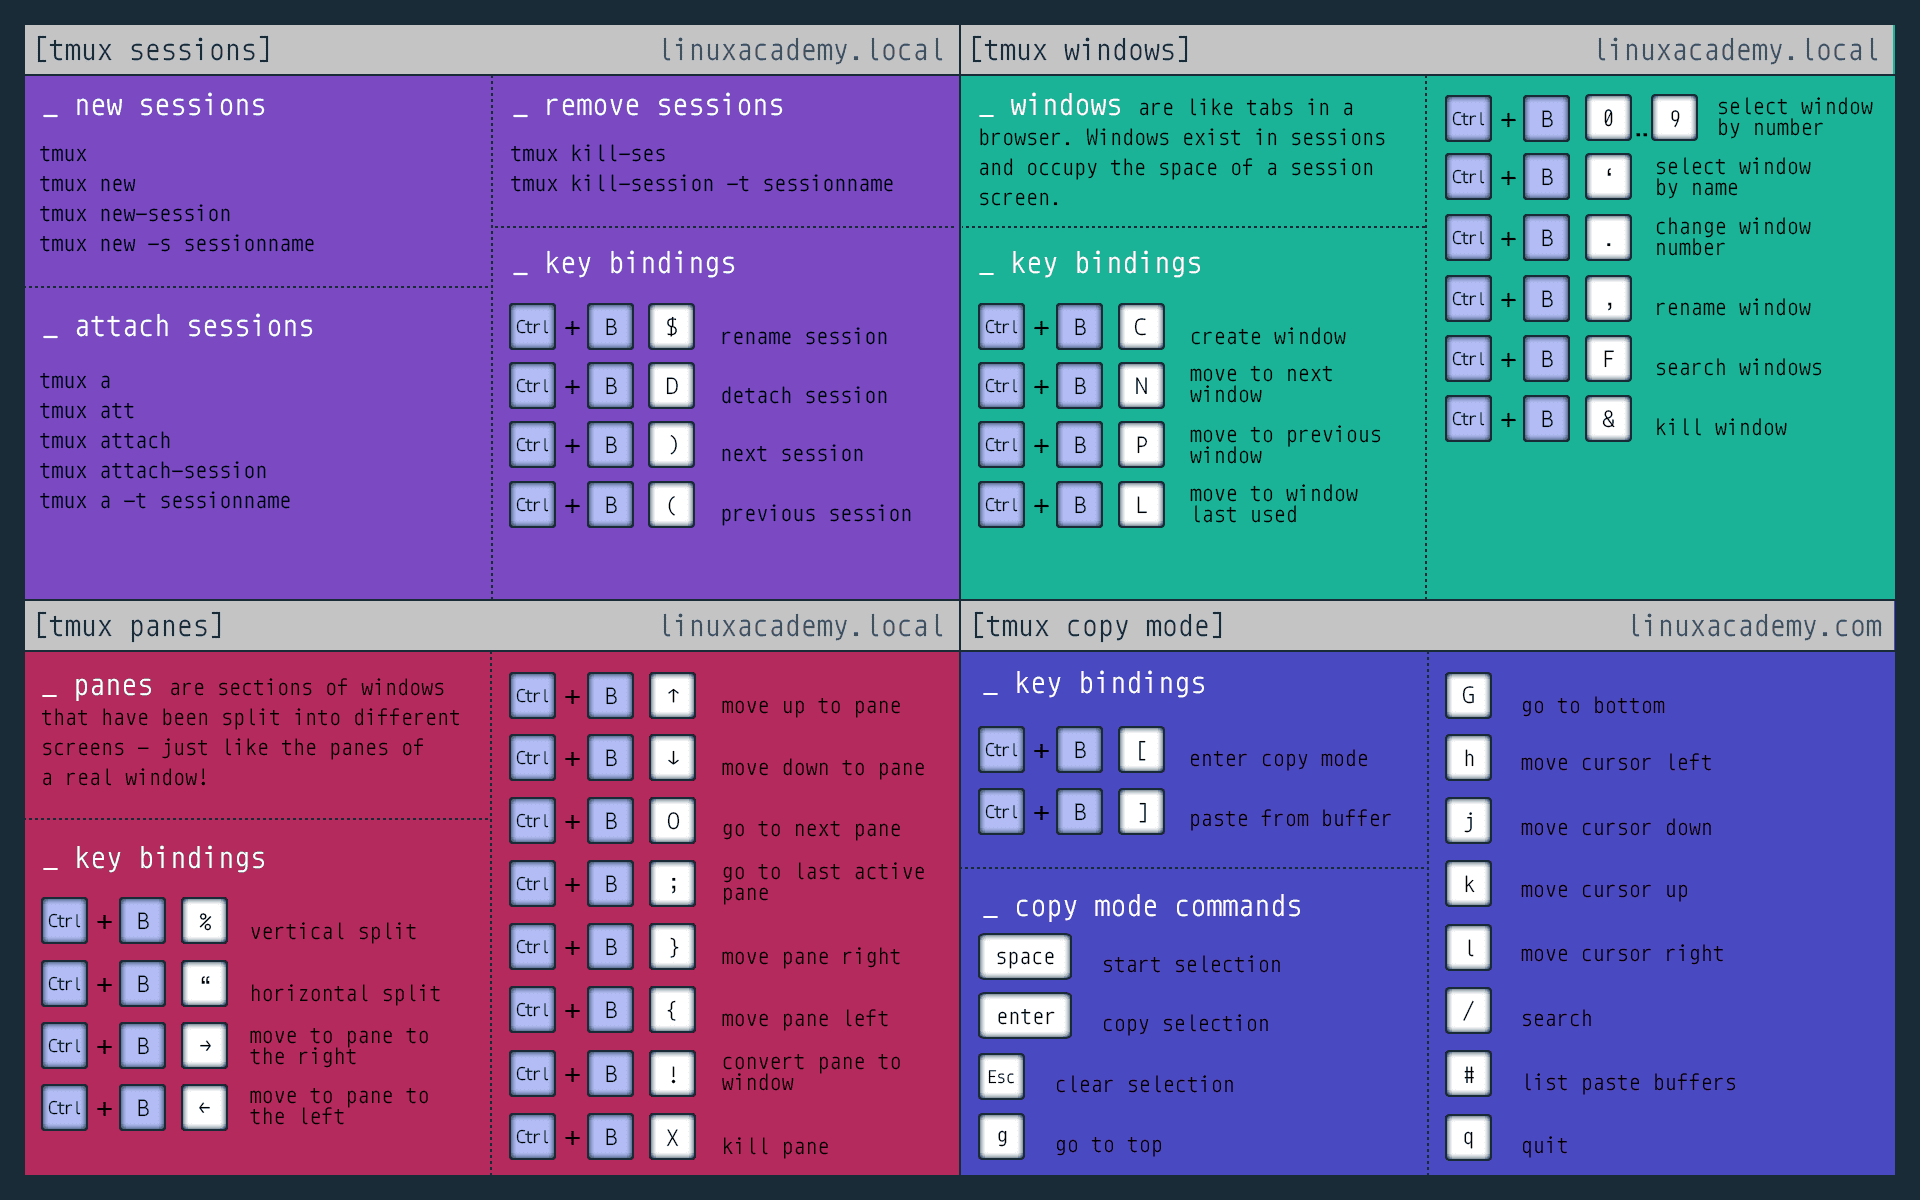
\includegraphics[width=\textwidth + 1.8cm, height=\textheight - 1cm]{graphics/tmux.png}
\end{frame}


\section{Ranger}
{ % all template changes are local to this group.
    \setbeamertemplate{navigation symbols}{}
    \begin{frame}<article:0>[plain]
        \begin{tikzpicture}[remember picture,overlay]
            \node[at=(current page.center)] {
                
\includegraphics[keepaspectratio,width=\paperwidth/4]{graphics/ra.png}
            };
        \end{tikzpicture}
     \end{frame}
}

\framesplit{Commander}{graphics/norton.png}{
    \begin{itemize}
        \item Norton - one of the very first \ex{dual pane file managers}, 1984
        \item Norton Commander set the tone for decades of file managers (Commanders) to come
        \item Until then people created nothing better than that, so DP commanders are still popular
        \item \ex{mc} (midnight commander) \hspace{2cm} \ex{dc} (double commander)
        \item There are a lot of both GUI and CLI examples, for Linux and Windows, but we will view cpecific one - \ex{ranger}
    \end{itemize}
}

\framesplit{Ranger}{graphics/ra_ex.jpeg}{
    \begin{itemize}
        \item Ranger is \ex{vim} inspired CLI file manager, so it has \ex{vi} keybindings
        \item It is fully customisible with just few files
        \item As you can see, it can open images preview right in the terminal
        \item The same about all text files, videos, other files too
        \item For more info see \ex{man ranger}
    \end{itemize}
}

\section{i3}
\framepic{graphics/i3wm.png}{i3wm}
\begin{frame}{i3}
    \begin{itemize}
        \item We will talk more about graphics in one of the folowing lectures
        \item Short explain: there are three main items in every GUI on your pc:
        \begin{itemize}
            \item \ex{DM} - Display manager
            \item \ex{WM} - Window manager
            \item \ex{DE} - Desctop envieronment
        \end{itemize}
        \item As you can see, \ex{i3wm} is a window manager
        \item It is quite similar to everything above in this lecture: vim shortcuts and tmux approach (but for GUI applications)
        \item In \ex{i3} we also have windows and panes, but also \ex{workspaces}
        \item All settings located in one file - \ex{~/.config/i3/config}
        \item As far as there is no DE for i3, you should install everything for yourself (all applets and programs, top/bottom bar, menu)
    \end{itemize}
\end{frame}

\framesplit{i3wm example}{graphics/myi3.jpg}{
    \begin{itemize}
        \item Here you can see browser and two terminal emulators opened
        \item Also \ex{polybar} with its applets used as top and bottom bars
        \item \ex{dmenu} used as a menu
        \item All windows located on a same \ex{z} level, new windows move previous one, so all opened windows are visible (as in \ex{TMUX})
        \item It is called \ex{tiling window manager}, and I recommend it because it is simpler and faster than all other types
        \item For more info you can see \ex{man i3}
    \end{itemize}
}

\section{Package managers}
\framepic{graphics/pacman.jpg}{Package 

managers}
\begin{frame}{Package managers}
    \begin{itemize}
        \item This is last but not least tool using on Linux based systems
        \item Any\ex{OS}is just a batch of programs communicating with each other
        \item And\ex{Package manager}is a tool for installing those programs (also upgrading, configuring, removing, resolving dependencies)
        \item Nice thing is that it is done in\ex{only one command}(with good package managers, not\ex[ucured]{apt}), not like in Windows OS (where pipeline looks like: find it somewhere, download, run some installation file, a lot of mouse movements and ugly GUI, then a lot of possible side applications are installed, and (probably) viruses)
        \item First, there are a few core new concepts that we need to understand how it works
    \end{itemize}
\end{frame}


\framesplitc{Mirrors}{graphics/mirror.png}{
    \begin{itemize}
        \item \ex{Mirror server (mirror)} - servers that located (phisically) in different locations, but contain the same data
        \item For example: You want to install something, but your internet connection is too slow (or something happend to server at the US), so you dounload package for installation from server located in Germany (or other location)
        \item See your current list of mirrors (Arch-based): \ex{vim /etc/pacman.d/mirrorlist}
        \item Sort them by speed: \ex{sudo fetchmirrors -c UA}
    \end{itemize}
}

\begin{frame}{Dependencies}
    \begin{itemize}
        \item Another core concept called \ex{dependency}
        \item When you write any program, you use some exsiting libraries. So your program \ex{depend on} that libraries/tools
        \item All that libraries have its versions
        \item As far as people change staff in their programs, API can be different from one to other version
        \item Good package managers can resolve all that dependencies easily (\ex{debian's apt can't})
        \item There are \ex{immidiet} (your program use it) and \ex{transitive} (your dependencies use it) dependencies
    \end{itemize}
\end{frame}

\framesplitc{Dependencies}{graphics/dependency.png}{
    \begin{itemize}
        \item A lot of programming languages has it's own package managers (\ex{pip} for Python, \ex{cargo} for Rust)
        \item Almost every Linux-based OS has it's own package manager 
        \item All packages are \ex{erchives} with \ex{program} itself and \ex{metadata} - software's name, description of its purpose, version number, vendor, checksum, list of dependencies
    \end{itemize}
}

\framesplit{Repositories}{graphics/repo.png}{
    \begin{itemize}
        \item One more important thing - repo
        \item There are official and side repositories
        \item Package manager supports Official repos by default, but to use some side repos, you should add it manually
        \item Defferent PacManagers have different approaches for managing repos
        \item \ex{Apt} repos are defined in \ex{/etc/apt/sources.list} and in \ex{/etc/apt/sources.list.d} directory
    \end{itemize}
}

\framesplit{Pacman}{graphics/pacman_archlinux.jpg}{
    \begin{itemize}
        \item Why we \ex{love}\ex[ucublue]{Arch Linux} so much? Mostly because of this guy =)
        \item \ex{Pacman} has all settings in \ex{/etc/pacman.conf} file
        \item Main repositories are:
        \begin{itemize}
            \item \ex{core} (main OS elements)
            \item \ex{extra} (not main, but important OS elements as GUI)
            \item \ex{community} (packages that have been adopted by Trusted Users from AUR)
            \item \ex{multilib} (32-bit software and libraries for old staff)
            \item \ex{AUR} (Arch User Repository, the best bigger Linux repo)
        \end{itemize}
    \end{itemize}
}

\begin{frame}{Releases}
    \begin{itemize}
        \item \ex{Release system} is the concept of frequently delivering updates to applications
        \item It usually depends on the OS (but also on PacManagers)
        \item \ex[ucuorange]{Rolling Release}. There is no such thing as \ex{Arch 1}, \ex{Gentoo 2} or \ex{Void Linux 3}. That's because these OS's have a Rolling Release model - its repos contain all (not always stable) new programs, but also previous versions of all packages. Good for people who like to test new programs or languages, real geeks. Often updates require
        \item \ex[ucuorange]{Stable Release}. A properly tested version of the product is released, sometimes half a year after it first appears. For example, \ex{python 3.9} was in \ex{pacman} two days after official release, but in \ex{apt} - more then half a year after. Good for average users, easy to maintain (updates are only every week/month)
        \item \ex[ucuorange]{LTS} - Long term support. For this system, package manager \ex{freeze} some special versions of all libraries and programs, and only \ex{minor bug or security fixes} are released for a long term (sometimes up to decades). Good for corporations, big companies. If something is not working - reinstall the system as it was at the very beginning, and everything will work again. The easiest to maintain
    \end{itemize}
\end{frame}


\section{Sources}
\framecard{Sources}
\begin{frame}{Sources}
    \begin{itemize}
        \item \href{https://www.linuxjournal.com/node/1203742}{Linux journal}
        \item \href{https://opensource.com/article/21/5/linux-terminal-multiplexer}{Termianl Multiplexers}
        \item \href{https://protechnotes.com/comprehensive-tmux-tutorial-for-beginners-with-a-cheat-sheet/}{Tmux tutorial}
        \item \href{https://man7.org/linux/man-pages/man1/tmux.1.html}{Tmux Linux man page}
        \item \href{https://fman.io/blog/dual-pane-file-manager-history/}{Dual pane file manager history}
        \item \href{https://github.com/ranger/ranger}{Ranger github page}
        \item \href{https://en.wikipedia.org/wiki/Package_manager}{Wiki package managers}
        \item \href{https://wiki.archlinux.org/title/pacman}{Pacman ArchWiki}
        \item \href{https://itsfoss.com/adding-external-repositories-ubuntu/}{External Repositories Ubuntu}
        \item \href{https://en.wikipedia.org/wiki/Rolling_release}{Releases Wiki}
    \end{itemize}
\end{frame}

\end{document}